\documentclass{cssotsuken}
\usepackage{amsmath}
\usepackage{amssymb}
\usepackage{amsfonts}
\usepackage[dvipdfmx]{graphicx}
\usepackage{here}
\usepackage[utf8]{inputenc}
\insert

\date{2019年10月 2日} % 西暦表記
\title{動画像圧縮ベース時系列分類手法のカラー情報を用いた改良}
\teacher{古賀 久志}
\mydata{1610333 下岡 藍人}

\begin{document}

\maketitle
\fontsize{10pt}{17pt}\selectfont

%↑ 上記は必須
%-----------以降,本文を記入-----------

%\vspace{10mm}
\section{はじめに}
近年、IoTなどの分野において時系列データを扱う事業が増加している。大量の時系列データを手動で分類することは多くのコストがかかるため、その自動化は重要なテーマである。圧縮ベースの分類手法の1つに、動画像圧縮技術を用いた、Recurrence Plots Compression Distance(RPCD)という手法がある。\cite{RPCD} この手法は、一般的な動画像圧縮ソフトを用いるため、だれでも手軽に利用できるという利点がある。RPCDでは時系列データの自己相関を表す、Recurrence Plot(RP)と呼ばれる画像を用いる。従来のRPCDではグレースケール画像を用いており、1つの画像につき1種類の情報しか画素値として格納できない。これは、グレースケールは輝度の情報しか保持していないためである。しかし、輝度のほかに色差信号の情報を持つカラー画像は3つのチャンネルを持つため、グレースケール画像よりも多くの情報を格納することができる。本研究の趣旨は、RPにより多くの情報を持たせることで、分類精度の向上を目指すというものである。


\section{RPCD}

本章ではRecurrence Plots Compression Distance(RPCD)について述べる。RPCD手法による2データ間の類似度計算の流れを図1に示す。RPCDではまず2つの時系列データからそれぞれRPと呼ばれる画像を生成し、それらを組み合わせた2つのフレームからなる動画像をMPEG-1で圧縮する。そこから得られるファイルサイズでデータの類似度を求め、データの分類を行う。

\begin{figure}[H]
	\centering
	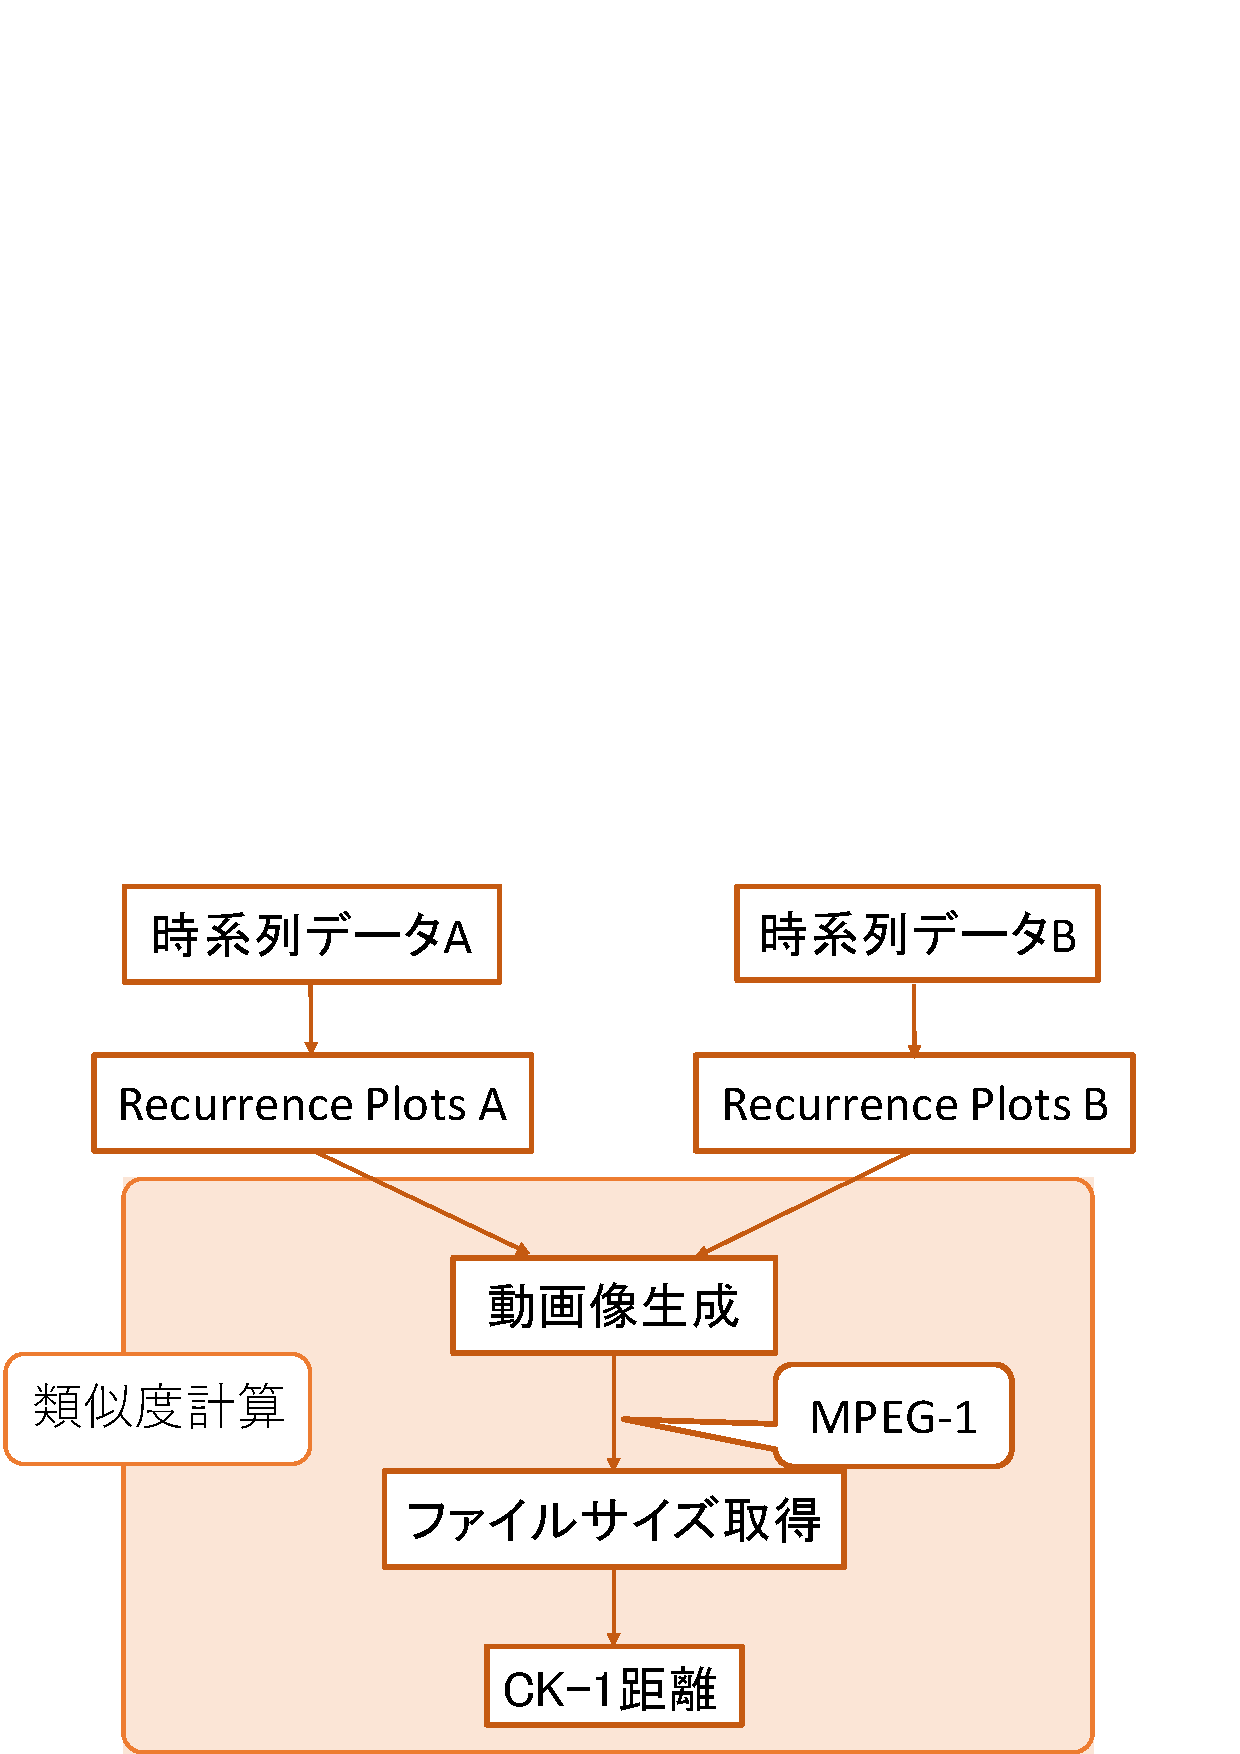
\includegraphics[width=7cm]{RPCD.png}
	\caption{RPCD手法の流れ}
	\label{fig:RPCD}
\end{figure}

\subsection{Recurrence Plot}

RPは以下の式\ref{RP1}で表される。
\begin{equation}
\label{RP1}
RP(i,j)=||\vec{x}(i)-\vec{x}(j)||, \vec{x}(\cdot)\in\mathbb{R}
\end{equation}
ここで,$\vec{x}(i)$は時系列データ$x$の$i$番目のサブシーケンスを表す.
得られたRPを正規化し,$RP(i,j)$の値を画素位置$(i,j)$の画素値とみなすことでグレースケール画像として表現できる.

\subsection{MPEG-1}
MPEG-1とは動画像圧縮規格の1つである。MPEG-1では圧縮対象のフレームの画素情報を直前のフレームから予測する、動き補償フレーム間予測を採用しており、これにより2つのフレームが似ているほど圧縮動画像のファイルサイズは小さくなる。

\subsection{CK-1距離}
CK-1距離とはCampanaらによって定義された、2画像間の類似度を動画像圧縮技術を用いて測る方法である。\cite{ck1} 2つの画像$x$,$y$が与えられたとき、その距離$D(x,y)$は以下の式\ref{CK1}で定義される。
\begin{eqnarray}
\label{CK1}
D(x,y)=\frac{C(x|y)+C(y|x)}{C(x|x)+C(y|y)}-1
\end{eqnarray}
ここで、$C(x|y)$は、1フレーム目が$y$、2フレーム目が$x$の動画像を圧縮した時のファイルサイズを表している。2画像が全く同じであるとき、$D(x,y)=0$となる。

\section{研究の目標と課題}
RPCD手法では動画像の圧縮にMPEG-1という規格を用いているが、このMPEG-1は元々カラーの動画像の圧縮を目的としている。つまり、RPとしてカラー画像を用いることも可能である。グレースケール画像では各ピクセルは輝度の情報しか持たないが、カラー画像では輝度の他に色差信号の情報を2つ持っている。この余った2チャンネルに何らかの情報を持たせることで、従来のRPよりも多くの情報を持ったRPを生成することが出来る。そこで、カラー情報を持つRPを生成し、情報量を増やすことで分類精度を向上させられるのではないかと考えた。しかしながら、RPにカラー画像を採用するにあたり以下の2点の問題がある。

\begin{enumerate}
\item 色空間の特性の問題
\item 新たに持たせる情報の種類を何にするか
\end{enumerate}

\subsection{色空間の特性}
  新たなRPの生成方法ではRGBではなくYCbCr色空間を用いる。これは、動画像圧縮の際、圧縮ソフトの内部でRGBからYCbCrに変換されるためである。RGBは赤、緑、青の3色の組み合わせで色を表現しているのに対し、YCbCrは輝度信号Yと、色の青さ、赤さを表す色差信号Cb,Crの組み合わせで表現している。RGBではR,G,Bそれぞれの画素値の範囲は$0\sim255$であり、どのような画素値の組み合わせでも色を表現できる。つまり色空間が立方体となっている。YCbCrではYの値域が$16\sim235$、Cb,Crの値域が$16\sim240$となっている。これはYCbCrからRGBに変換する際、RGBの色空間からはみ出てしまうことがあり、それを避けるためである。さらにこの値域の内部であっても、画素値の組み合わせ次第ではRGBの色空間をはみ出てしまう。このことから、それぞれの値域を定める必要があるが、YCbCrそれぞれの値域は独立ではなく、一つの値域を広くすると他の値域が狭まってしまうという特性があり、慎重に調整する必要がある。
\subsection{追加する情報の種類}
新RPでは、輝度Yには従来と同じ情報を格納し、色差Cb,Crに新たに何らかの情報を格納することになるが、具体的にどのような情報を持たせるかが重要となる。

\section{実験および結果}
\subsection{実験内容と方法}
新たに持たせる有用な情報を探すため、Crの値を固定し、Cbに様々な情報を持たせ分類精度を測定している。一例として、Cbに時系列データの絶対値を持たせた際の分類結果を紹介する。従来のRPでは時系列データの各時間同士の差分を取っているため、絶対値の情報が失われている。そこで、Cbに絶対値の情報を持たせることは有用ではないかと考えた。実験にはUCR Time Series archiveから12個のデータセットを使用した。動画像圧縮ソフトにはFFmpegを使用し、絶対値情報を持たせない場合と比較を行った。
\subsection{結果}
Cbに絶対値を入れたRPの分類精度を絶対値情報を持たせない場合と比較した。実験結果を表\ref{ta:hikaku}に示す。表1より、12個のデータセットのうち精度が向上したものは4つのみであり、平均はおよそ1\%低下した。全体としては下がっているものの、もし訓練データからテストデータの結果を予測できれば、データセットによって持たせる情報を切り替えることで精度を向上させられる可能性もあると考えている。

\section{まとめ}
本研究では従来の動画像圧縮ベースの時系列分類手法をベースに、カラー画像を採用することで精度の向上を目指すことを目標としている。今後は新たに格納する情報を模索していく予定である。

\begin{table}[t]
	\small
	\caption{分類精度}
	\label{ta:hikaku}
    \begin{center}
	\begin{tabular}{lccc}
		\hline
		dataset&絶対値情報あり&なし\\
		\hline
		\hline
		Beef&56.67&\bf{63.33}\\
		Coffee&\bf{100}&\bf{100}\\
		ECG200&\bf{91.00}&89.00\\
		FISH&92.00&\bf{95.43}\\
		FaceFour&\bf{96.59}&95.45\\
		Gun Point&\bf{100}&\bf{100}\\
		ItalyPoserDemand&\bf{95.14}&94.85\\
		Lighting2&73.77&\bf{75.41}\\
		Lighting7&\bfseries{65.75}&58.90\\
		OliveOil&83.33&\bfseries{90.00}\\
		SonyAIBORobot&84.69&\bfseries{85.69}\\
		Symbols&95.23&\bfseries{97.49}\\
		\hline
		Best&6/12&\bf{8}/12\\
		Average&86.18&\bfseries{87.13}\\
		\hline
	\end{tabular}
    \end{center}
\end{table}


\begin{thebibliography}{99}
\bibitem{RPCD}
G. D. B. Silva and V. de Souza, “Time Series Classification
using compression distance of recurrence plots,” in Proc.
IEEE 13th Int. Conf. Data mining, pp. 687-696, 2013.

\bibitem{ck1}
B. J. L. Campana and E. J. Keogh, ``A Compression Baseed Distance Measure for Texture,'' in Proc.  the 10th SIAM International Conference on Data Mining, pp. 850-861, 2010.

\end{thebibliography}

\end{document}